\section{Strumentazione}
	Per effettuare tale misurazioni abbiamo impiegato:

	\begin{itemize}
		\item l'apparato e/m PASCO SE-9638 composto da:
		\begin{itemize}
			\item un bulbo di vetro contenente Neon alla pressione di $10^{-2} \; \si{\mmHg}$;
			\item un cannone elettronico all'interno del bulbo: un catodo riscaldato che emette elettroni, che vengono poi accelerati dal potenziale applicato tra catodo e anodo;
			\item due bobine di Helmholtz di raggio \SI{15}{cm} e 130 spire, che generano il campo magnetico;
		\end{itemize}
		\item alimentatori per regolare la tensione $V$ del cannone elettronico e la corrente $I$ passante per le bobine, queste grandezze vengono misurate dagli stessi e sono note con una risoluzione rispettivamente di \SI{1}{V} e $ $\SI{0.01}{\ampere};
		\item un sensore di Hall SS94A, per la misura del campo magnetico e un circuito per la sua calibrazione e lettura;
		\item una macchina fotografica digitale, per l'acquisizione delle tracce prodotte dagli elettroni, urtando ed eccitando gli atomi di elio;
		\item Un righello retroilluminato di risoluzione \SI{1}{\mm} che verrà usato per calibrare la misura dei raggi;
		\item un metro di risoluzione \SI{1}{\mm} usato per correggere la prospettiva poiché il piano del righello non coincide con quello dove si muovono gli elettroni.

In \figurename{ \ref{apparato}} è mostrato uno schema dell'apparato di misura.

	\begin{figure}[H]
		\centering
		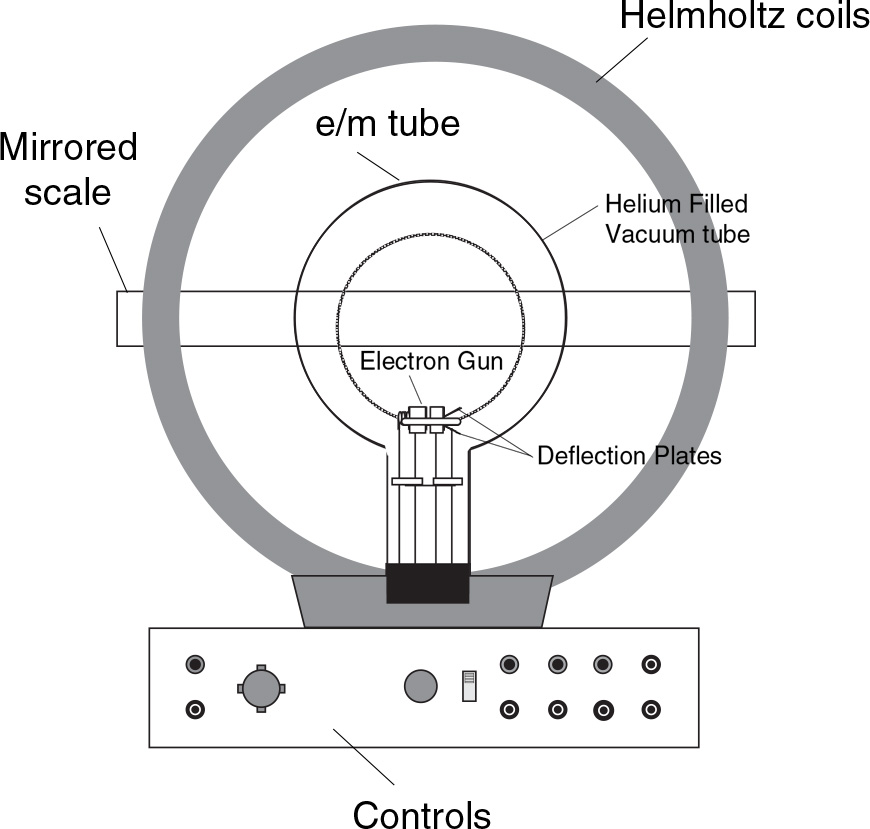
\includegraphics[scale=1.4]{apparato.jpg}
		\caption{apparato di misura}
		\label{apparato}
	\end{figure}

	\end{itemize}

\section{Misure da effettuare}
Gli elettroni vengono accelerati dal campo presente nel cannone elettronico e se lo strumento fosse perfetto (torneremo in seguito su questo punto) dovrebbero uscirne con velocità $v = \sqrt{2V \sfrac{e}{m} }$, che quindi dipende solo dal potenziale $V$.
Il campo magnetico esercita una forza centripeta pari a $F = evB = mv^2/r$, segue che $$\frac{e}{m}=\frac{2V}{(B r)^2}.$$

\noindent Bisognerà procedere alle seguenti misure:
\begin{itemize}
	\item misura di \textbf{B}: fissata la geometria delle bobine di Helmholtz il campo magnetico è teoricamente ricavabile a partire dalla sola intensità di corrente $I$. Si procederà alla misura del campo magnetico per mezzo del sensore di Hall al variare di $r$ per testarne l'uniformità e si fitterà la legge teorica. Successivamente nella misura di $\tfrac{e}{m}$ ci si limiterà alla misura di $I$ e al calcolo di $B$ a partire dalla legge fittata;
	\item misura di \textbf{r} (raggio di curvatura degli elettroni): è determinato a partire da foto acquisite con un macchina fotografica digitale; la conversione pixel/metri deve tener conto dell'effetto prospettico dovuto alla diversa distanza a cui si trovano il righello di riferimento e il piano degli elettroni, bisognerà inoltre valutare l'effetto di distorsione dovuto al bulbo di vetro;
	\item misura di \textbf{V}: da questa dipende la velocità di uscita degli elettroni ed è letta direttamente dall'alimentatore del cannone elettronico con una risoluzione di \SI{1}{\volt}; nel corso dell'esperienza misureremo il raggio di curvatura al variare di $V$ tra \SI{200}{\volt} e \SI{300}{\volt}.
\end{itemize}
\newpage
\section{Misura di \textbf{B}}
Essendo l'apparato sensibile al campo magnetico terrestre, con una bussola si è individuata l'orientazione di $B_{\earth}$ e si sono orientate le bobine in modo da minimizzarne l'influenza, ovvero ponendo l'asse delle bobine in direzione ortogonale a $B_{\earth}$. Così facendo l'influenza di quest'ultimo sul moto circolare degli elettroni si riduce ad una piccola forza in direzione assiale, che introduce una lieve non planarità della traiettoria, essenzialmente ininfluente sulla successiva analisi dati, dal momento che piccole differenze di profondità nella traccia dell'elettrone non risultano in un raggio di curvatura diverso.

\paragraph{} La sonda ad effetto Hall necessita inoltre della calibrazione dello zero: si è perciò andati a modificare gli offset del circuito di amplificazione della sonda, agendo sul potenziometro del circuito sino a quando non si ottenesse una lettura uguale in modulo (e opposta in segno) in seguito ad una rotazione di \ang{180} della sonda.

Effettuato ciò si sono alimentate le bobine con una tensione $V_{coil}= \SI{7.5 \pm 0.1}{\volt}$ ottenendo una corrente $I=\SI{0.95 \pm 0.01}{\ampere}$\footnote{Tali misure sono ottenute dalla lettura del generatore di tensione; si è assunto come errore un digit, a cui andrebbe aggiunto l'errore (ignoto) di calibrazione dell'apparato.}; dopodiché si è mappato il campo $B_z$ sul piano del moto degli \e in funzione della distanza dal centro dell'apparato per un intorno di $\sim $\SI{\pm 6}{\cm}.
Si è ritenuta tale regione come area di interesse poiché si essendo il raggio del bulbo approssimativamente di \SIrange{5}{6}{\cm}, il moto gli elettroni osservabili si svolge certamente entro tale intervallo.

La sonda restituisce un segnale in tensione che è amplificato con un guadagno noto
$G = \num{11.090(3)}$ e viene letta attraverso un multimetro in dotazione. Si è associata alla lettura un incertezza di mezzo digit.

La posizione della sonda è identificata dalla distanza $l$ di un'estremità dell'asta che la contiene dal lato dell'apparato attraverso cui l'asta è infilata; è stato eseguito un fit per determinare la posizione $l_0$ corrispondente al centro.

I valori ottenuti da tale mappatura sono riportati in appendice in \tablename{ \ref{tab:a}}.

Dai dati tabulati si è ricavato $B_z$, tenendo conto dell'amplificazione e della risposta della sonda (\SI{5.0(1)}{\mV\per\gauss}); i dati sono mostrati in \figurename{ \ref{fig:fit1}}: è chiaro l'effetto della digitalizzazione della tensione in uscita dalla sonda. È inoltre riportato l'andamento ottenuto da un fit a tre parametri della formula (valida lungo il piano equidistante dalle due bobine):
\begin{equation} \label{eq:bz}
		B_z = \frac{\mu_0 N I}{4 \pi} \int_0^{2\pi} \frac{2\, R\, (R - r \cos\theta )}{\big(\frac{5}{4} R^2 + r^2 + 2\, R \, r \cos \theta\big) ^ {3/2}} \, \dd \theta
\end{equation}
Dove $I$ è la corrente nelle spire delle bobine, $N$ il numero di avvolgimenti, $\mu_0$ la permeabilità magnetica del vuoto, $R$ il raggio delle bobine ed $r = |l - l_0|$ la distanza dall'asse delle bobine.


\begin{figure}[H]
	\centering
	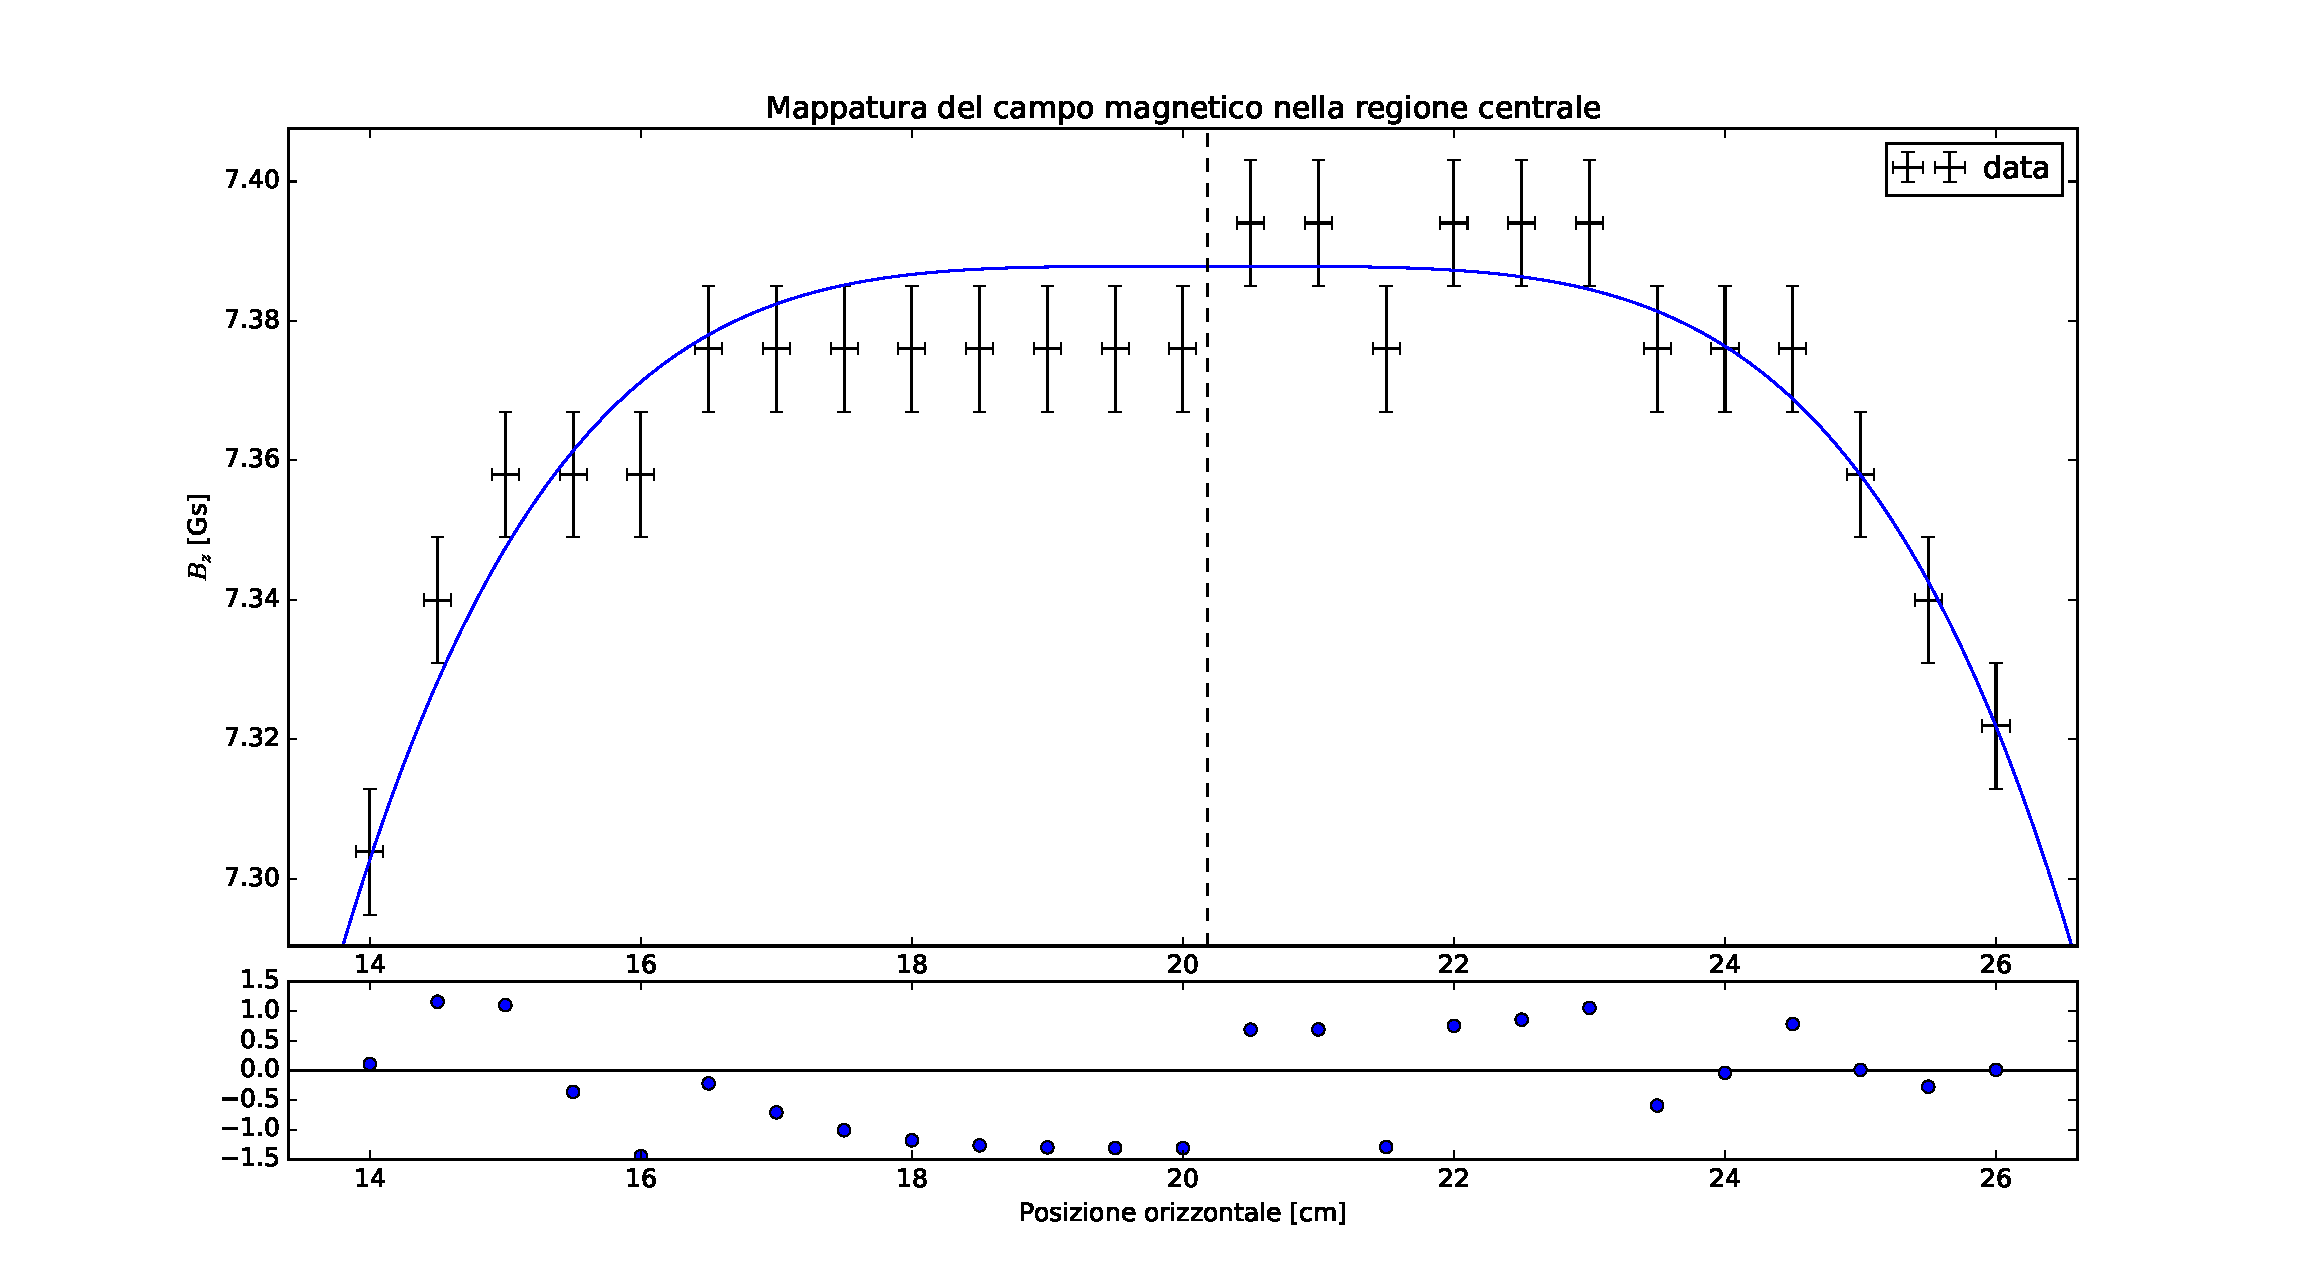
\includegraphics[scale=0.45]{mappatura_bz.pdf}
	\caption{Mappatura e fit.}
	\label{fig:fit1}
\end{figure}

Dal fit si sono ricavati la posizione $l_0 = \SI{20.2(2)}{\cm} $, il raggio delle bobine $R = \SI{15.9(8)}{\cm}$ ed un fattore correttivo $k = \num{1.06(5)}$ al prodotto $N I$ (ovvero un fattore tale che $N I$ utilizzato in \eqn{bz} sia pari a $k \, (N I)_{nominale}$, dove il fattore nominale viene calcolato dal valore indicato per il numero di avvolgimenti e la corrente misurata dal generatore ed è dunque pari a $130 \cdot  \SI{0.95}{\A}$); si ottiene $\chi^2 = 19.7 \ (22 \dof , \  p = 0.60)$.

I valori non sono lontani da quanto atteso, ma potrebbero indicare un'inesattezza nel numero di avvolgimenti oppure un errore di calibrazione dell'amperometro dell'ordine del \%, oltreché un raggio medio delle bobine leggermente diverso da quanto indicato (sebbene quest'ultima discrepanza possa essere data anche dalla distanza dalle bobine, che compare nella formula per $B_z$ anch'essa come $R$ ma che potrebbe essere diversa, ed inoltre avendo le bobine una certa larghezza potrebbe non essere pienamente trascurabile la deviazione dall'approssimazione che le vede come anelli).

Per il campo magnetico al centro dell'apparato in funzione della corrente si ottiene, utilizzando i parametri fittati per determinare $B_z(r=0)$ e dividendo per la corrente misurata (\SI{0.95(1)}{\A}), $B_{z,max} = \SI{7.77(15)}{\gauss\per\A} \, \cdot \, I$.
Così facendo, utilizzando questo dato per calcolare in seguito $B_z$ al variare di $I$ dovremmo escludere l'eventuale errore di calibrazione dell'amperometro (assumendo che il suo zero sia invece sufficientemente preciso).
